\documentclass[letterpaper,journal]{IEEEtran}
\usepackage{amsmath,amsfonts}
\usepackage{algorithmic}
\usepackage{algorithm}
\usepackage{array}
\usepackage[caption=false,font=normalsize,labelfont=sf,textfont=sf]{subfig}
\usepackage{textcomp}
\usepackage{stfloats}
\usepackage{url}
\usepackage{verbatim}
\usepackage{graphicx}
\usepackage{cite}
\hyphenation{op-tical net-works semi-conduc-tor IEEE-Xplore}
% updated with editorial comments 8/9/2021

\begin{document}

\title{NUFROST: Robust Reconstruction of Irregularly Sampled Optical Remote Sensing Time Series}

\author{Luhao Yang, ..., and Hui Fan*%
\thanks{Corresponding author: Hui Fan (e-mail: fanhui@ynu.edu.cn).}%
}

% The paper headers
\markboth{Journal of \LaTeX\ Class Files,~Vol.~14, No.~8, August~2021}%
{Shell \MakeLowercase{\textit{et al.}}: A Sample Article Using IEEEtran.cls for IEEE Journals}

\IEEEpubid{0000--0000/00\$00.00~\copyright~2021 IEEE}
% Remember, if you use this you must call \IEEEpubidadjcol in the second
% column for its text to clear the IEEEpubid mark.

\maketitle

\begin{abstract}
Optical remote sensing time series are crucial for monitoring land surface dynamics, but they often suffer from irregular sampling, cloud-driven gaps, residual contamination, and abrupt land-surface events. This study introduces NUFROST, a robust reconstruction framework that combines Non-Uniform Fast Fourier Transform (NUFFT) spectral estimation with a step-preserving harmonic reconstruction model. NUFROST estimates the spectrum of non-uniformly sampled pixels without interpolation, identifies dominant seasonal frequencies through adaptive selection and parabolic refinement, and reconstructs multi-band reflectance using frequency-tiered Ridge regression coupled with a group fused-lasso step term. The harmonic component captures low- and medium-frequency phenological structure, while the sparse piecewise-constant innovation term preserves shared abrupt changes across spectral bands without forcing them into globally oscillatory high-frequency Fourier bases. Experiments on Sentinel-2 Harmonized time series demonstrate that NUFROST outperforms traditional harmonic and regression-based methods in both sparse-observation and continuous-gap scenarios, providing a practical solution for reliable temporal analysis in complex environments.
\end{abstract}

\begin{IEEEkeywords}
Time Series Reconstruction, Non-Uniform FFT, Fused Lasso, Remote Sensing, Sentinel-2
\end{IEEEkeywords}

\section{Introduction}
\IEEEPARstart{O}{ptical} satellite image time series provide a fundamental data source for monitoring vegetation phenology, land-cover dynamics, and disturbance processes over large spatial extents~\cite{ref1,ref2}. With the increasing availability of dense Sentinel-2 observations, sub-seasonal land-surface variation can in principle be reconstructed at high spatial resolution. In practice, however, the usable observations remain highly irregular because cloud, snow, shadow, atmospheric contamination, and sensor-viewing conditions remove a large fraction of acquisitions. This problem is particularly severe in mountainous and humid regions, where persistent cloud cover and complex terrain lead to long temporal gaps and uneven observation density.

Reconstructing such irregular optical time series is challenging for three reasons. First, conventional Fourier and harmonic models are naturally defined on uniformly sampled signals. Therefore, irregular observations are often interpolated or smoothed onto a regular temporal grid before frequency-domain analysis. This preprocessing may introduce artificial periodicity across long gaps and distort the spectral content of the original observations~\cite{ref5}. Second, residual thin clouds and atmospheric artifacts can produce large but temporally localized deviations. Least-squares harmonic fitting tends to absorb these deviations into global sinusoidal components, causing ringing and unstable extrapolation. Third, abrupt land-surface events, such as harvest, disturbance, or rapid vegetation change, are not well represented by purely smooth harmonic bases. Increasing the number of high-frequency components improves local flexibility but also amplifies overfitting under sparse observations.

Existing reconstruction methods address parts of this problem but not the complete setting. HANTS~\cite{ref10} provides an efficient harmonic reconstruction framework and can suppress isolated outliers, but its Fourier representation is most stable under relatively regular temporal support. Regression and segmentation-based methods, including the Zhu2015 approach~\cite{ref14}, improve flexibility by fitting temporal basis functions or local segments, but their performance can degrade when the number of valid observations in a segment becomes small. More broadly, interpolation-based preprocessing and purely harmonic reconstruction both struggle to separate persistent local changes from globally oscillatory seasonal structure.

To address these limitations, we propose NUFROST (Non-Uniform FFT-based Reconstruction of Optical Satellite Time-series), a reconstruction framework for irregularly sampled optical remote sensing time series. NUFROST first estimates the spectral structure of valid observations directly on their original non-uniform acquisition times using the Non-Uniform Fast Fourier Transform (NUFFT), avoiding temporal interpolation before frequency estimation~\cite{ref4,ref6}. The selected dominant frequencies define a compact harmonic basis for stable phenological variation. The final reconstruction then combines frequency-tiered Ridge regularization with a sparse step component. Low- and medium-frequency harmonics are retained to model seasonal dynamics, while unreliable high-frequency oscillations are penalized more strongly. Persistent abrupt changes are represented by a fused-lasso step term rather than forced into global Fourier bases~\cite{ref9,ref15}. The main contributions of this work are summarized as follows:

\begin{enumerate}
    \item We introduce a NUFFT-based spectral estimation strategy for irregular optical satellite observations, enabling dominant seasonal frequencies to be identified without first regularizing the time axis by interpolation.
    \item We develop a frequency-tiered harmonic reconstruction model that stabilizes high-frequency components under sparse and gapped observations while preserving the low-frequency phenological backbone.
    \item We formulate a step-preserving sparse reconstruction term for persistent local changes, allowing abrupt events to be separated from smooth seasonal variation and reducing harmonic ringing in difficult gap-filling cases.
\end{enumerate}

Experiments on Sentinel-2 Harmonized time series across multiple AOIs and six spectral bands compare NUFROST with HANTS~\cite{ref10} and Zhu2015~\cite{ref14} under sparse-observation and continuous-gap settings. The results show that NUFROST provides more accurate and stable reconstruction, especially when valid observations are unevenly distributed or prolonged temporal gaps are present.

\IEEEpubidadjcol
The remainder of this paper is organized as follows. Section~II reviews related work on optical time-series reconstruction. Section~III presents the proposed NUFROST model, including NUFFT-based frequency estimation, dominant-frequency selection, and step-preserving reconstruction. Section~IV describes the experimental setup and results. Section~V concludes the paper.

\section{Background and Related Work}
Optical remote sensing time series are widely used to characterize land-surface dynamics, including vegetation phenology, forest disturbance, and ecological change~\cite{ref1,ref2}. In these applications, temporally consistent reflectance trajectories are often a prerequisite for reliable downstream analysis. However, optical observations are frequently contaminated by clouds, cloud shadows, snow, and atmospheric variability. After quality masking, the remaining valid observations are usually irregularly distributed in time and may contain long gaps, especially in humid and mountainous regions where persistent cloud cover further reduces observation continuity~\cite{ref3,ref13}.

A large body of work has attempted to improve the temporal consistency of optical time series through interpolation, smoothing, and curve-fitting strategies. Simple interpolation and smoothing filters can efficiently produce regularly sampled trajectories, but they may oversmooth short-term variations or introduce artificial temporal patterns when observations are sparse~\cite{ref4}. Harmonic-based methods, such as HANTS~\cite{ref10}, are effective for representing seasonal signals and suppressing random noise when temporal sampling is sufficiently dense. Nevertheless, conventional Fourier or harmonic analysis is naturally formulated on uniformly sampled observations. Therefore, irregular optical time series are often regularized by interpolation or gap filling before frequency-domain modeling, which may alter the original spectral structure and generate pseudo-periodic components across long missing intervals~\cite{ref5}.

Regression-based and temporal-segmentation approaches provide another line of research. Methods such as LandTrendr~\cite{ref11} and CCDC~\cite{ref12} model temporal trajectories using piecewise trends or harmonic components and have been widely used for disturbance detection and land-cover change analysis. The Lasso-based fitting algorithm proposed by Zhu et al.~\cite{ref14} improves the flexibility of reflectance prediction by selecting suitable temporal basis functions from available observations. Because Zhu2015 segments the time series at detected breaks and fits a separate Lasso model per segment, the effective number of observations per fit can become quite small. Under sparse sampling, the per-segment Lasso optimizer frequently reaches the maximum iteration limit without satisfying the convergence tolerance, so the harmonic coefficients may be sub-optimally estimated---a limitation that worsens at higher model orders and for segments with fewer than approximately 15 clear observations. However, these methods rely on the stability of the input temporal trajectory. With sparse observations, residual thin clouds, or atmospheric scattering, fitting can become sensitive to high-frequency fluctuations and outlying observations, leading to biased reconstruction and unstable change analysis~\cite{ref7}.

Non-uniform spectral estimation provides a promising alternative for irregularly sampled time series. Instead of forcing valid observations onto a regular temporal grid, the Non-Uniform Fast Fourier Transform (NUFFT) estimates spectral components directly from non-uniform observation times~\cite{ref4,ref6}. This property is particularly relevant for optical satellite time series, where the sampling pattern is determined by both revisit cycles and quality masking. However, NUFFT alone only provides a spectral representation; it does not by itself suppress residual atmospheric outliers, prevent high-frequency overfitting under severe temporal gaps, or localize abrupt events. Robust statistical screening and regularization are therefore necessary for converting non-uniform spectral information into stable pixel-wise trajectories~\cite{ref8,ref9}. Sparse and piecewise-constant regularization, such as fused-lasso penalties, offers a complementary way to represent persistent local changes without expanding the global Fourier basis~\cite{ref15}.

Motivated by these limitations, this study develops NUFROST, a framework that combines NUFFT-based frequency estimation with frequency-tiered Ridge fitting, joint multi-band outlier screening, and group fused-lasso step reconstruction. The framework avoids interpolation-induced spectral distortion by estimating spectra directly from irregular observations, regularizes unreliable high-frequency components, and explicitly assigns persistent abrupt changes to a local step term instead of forcing them into globally oscillatory harmonic components.

\section{Proposed Method}
The proposed NUFROST algorithm provides a robust framework for reconstructing optical remote sensing time series from irregular observations. The method is composed of three stages: (1) accurate frequency estimation from non-uniformly sampled time series using the Non-Uniform Fast Fourier Transform (NUFFT), (2) hybrid dominant-frequency selection with optional preferred seasonal periodicities, and (3) multi-band trajectory reconstruction using a frequency-tiered harmonic component and a sparse step component. The harmonic component models stable phenological variation, whereas the step component captures persistent abrupt events, such as harvest, fire, or land-cover change, without using globally oscillatory high-frequency Fourier terms. Before the final optimization, a joint multi-band outlier screen removes time steps with correlated residual anomalies, reducing color inconsistency caused by band-specific cloud contamination.

\subsection{Non-Uniform FFT}

Remote sensing image time series in complex mountainous environments commonly suffer from irregular sampling, missing observations, and noise interference, which directly affect the reliability of temporal change detection. Traditional Fast Fourier Transform (FFT) methods strictly require uniformly sampled data. When dealing with remote sensing data missing pixels due to cloud and snow removal, conventional approaches frequently employ methods like linear interpolation or Savitzky-Golay filtering to regularize the time axis before performing FFT. However, such interpolation methods tend to significantly alter the spectral characteristics of the original signal, for example, by introducing pseudo-periodicities at long temporal gaps or amplifying noise in the high-frequency band.

To address this problem and directly compute the spectrum from non-uniformly sampled data, this study introduces the Non-Uniform Fast Fourier Transform (NUFFT)~\cite{ref4,ref6}. By avoiding interpolation entirely, NUFFT prevents spectral distortion. The basic idea of NUFFT is to establish a connection between non-uniform sampling points and a uniform grid, and then use fast algorithms to approximately calculate the exponential sums, thereby maintaining a computational complexity comparable to standard FFT.

The core computational process typically involves three steps: first, the irregular sampling points are spread to an oversampled regular grid via a local kernel function, a process known as ``spreading" or ``convolution"; subsequently, a standard Fast Fourier Transform (FFT) is executed on this regular grid; finally, the result is corrected by deconvolution to recover the true Fourier coefficients.

Assuming an irregularly sampled time series of a remote sensing image pixel consists of $M$ samples, the tuple of time and reflectance at that time is represented as $(t_j, y_j)_{j=1}^M$. Through linear normalization, the sampling times are mapped to $[-\pi, \pi)$. Let $x_j = \frac{2\pi}{T}(t_j - t_0) - \pi$ and $c_j = y_j$, where $T$ is the total duration of the time series. In actual computation, to leverage the fast grid operations, the irregular sampling is viewed as a pulse sequence, as shown in Eq.~(\ref{eq:pulse}), where $\delta(x)$ is the Dirac impulse function.

\begin{equation}
\label{eq:pulse}
\mu(x) = \sum_{j=1}^{M} c_j \delta(x - x_j)
\end{equation}

Based on this, a compactly supported periodic kernel function is introduced, such as the Kaiser-Bessel (KB) kernel. This function realizes the grid mapping from non-uniform sampling points to uniform sampling through convolution, possessing finite support, low sidelobes, and numerical stability. Here, the selected kernel function and the periodized kernel function are denoted as $\psi(x)$ and $\psi_{per}(x)$ respectively, and their relationship is shown in Eq.~(\ref{eq:kernel}). The periodized kernel function is the periodic extension of the kernel function, used to prevent boundary overflow during convolution.

\begin{equation}
\label{eq:kernel}
\psi_{per}(x) = \sum_{m \in \mathbb{Z}} \psi(x - 2\pi m)
\end{equation}

By convolving the input time series with the kernel function, a uniformly sampled time series can be obtained:

\begin{equation}
\label{eq:conv}
b_l = (\mu * \psi)(lh) = \sum_{j=1}^{M} c_j \psi(lh - x_j), \quad l = 0, ..., n - 1
\end{equation}

where $h = \frac{2\pi}{n}$ is the uniform grid step size, and $l$ is the grid index. At this point, the traditional FFT can be used to perform time-frequency transformation on the time series with a uniform step size. The FFT calculation is shown in Eq.~(\ref{eq:fft}):

\begin{equation}
\label{eq:fft}
\hat{b}_k = \sum_{l=0}^{n-1} b_l e^{-2\pi i k l / n}, \quad k \in I_n = \{-\frac{n}{2}, ..., \frac{n}{2}-1\}
\end{equation}

The obtained $\hat{b}_k$ is the discrete spectrum corresponding to the uniform time series. Similarly, FFT can be performed on the periodic kernel function to obtain the discrete spectrum of the kernel function $\hat{\psi}_k = \text{FFT}\{\psi_l\}$. Since $f * h = \hat{f} \cdot \hat{h}$, the spectrum $\hat{f}_k$ of the original signal can be recovered through deconvolution correction via Eq.~(\ref{eq:deconv}).

\begin{equation}
\label{eq:deconv}
\hat{f}_k = \frac{\hat{b}_k}{\hat{\psi}_k}, \quad k \in I_n = \{-\frac{n}{2}, ..., \frac{n}{2}-1\}
\end{equation}

Through the three steps of convolutional spreading, fast Fourier transform, and deconvolution correction, spectral estimation for non-uniform sampling can be achieved. The discrete spectrum $\hat{f}_k$ contains the complete information of the original irregular time series. However, remote sensing time series are often affected by multiple sources of noise, and the spectral components of noise are also mixed in the current discrete spectrum. To fit the time series of true surface reflectance, a method that can effectively eliminate the noise components is needed.

\subsection{Step-Preserving Harmonic Reconstruction}

To reconstruct true surface reflectance while suppressing residual contamination, NUFROST first identifies the dominant frequency components from the NUFFT spectrum and then separates each multi-band pixel trajectory into a harmonic seasonal component and a sparse persistent step component.

\subsubsection{Dominant Frequency Selection}
The discrete spectrum $\hat{f}_k$ obtained from NUFFT contains both physical periodic variations (e.g., phenology) and observational noise. We select the dominant frequencies using a hybrid strategy that combines prior phenological knowledge with data-driven spectral peaks. The spectral power for each frequency component is defined as:
\begin{equation}
\label{eq:power}
P_k = \left|\hat{f}_k\right|^2
\end{equation}

First, to ensure robust extraction of stable seasonal phenology, we introduce preferred prior frequencies (e.g., annual and semi-annual cycles). These target frequencies are snapped to the nearest valid local maxima in the spectrum within a relative tolerance $\epsilon_{tol}$, preventing the model from missing the core phenological backbone due to noise interference.

Next, to capture region-specific or interannual variations, we supplement the selection with a data-driven peak picking process. We filter out the DC component and extremely low frequencies, restricting the candidate frequencies to $K_+ = \{k \in I_n \mid \nu_k \ge \nu_{min}\}$, where $\nu_k = k/T$ and $\nu_{min}$ is a minimum frequency threshold. The remaining spectral peaks are sorted in descending order of their power. We select the top peaks until their cumulative energy exceeds a predefined threshold $\eta$.

Since the NUFFT evaluates the spectrum on a discrete frequency grid, the true peak frequencies may lie between grid points. To improve estimation accuracy, we apply parabolic refinement around the local maxima. For a detected peak at frequency bin $i$ with power $P_i$, the refined frequency $\tilde{\nu}_i$ is obtained by interpolating with its adjacent bins:
\begin{equation}
\label{eq:parabolic}
\tilde{\nu}_i = \nu_i + \frac{1}{2}\frac{P_{i-1} - P_{i+1}}{P_{i-1} - 2P_i + P_{i+1}} (\nu_{i+1} - \nu_i)
\end{equation}
This hybrid selection yields a final set of refined dominant frequencies $\Omega = \{\tilde{\nu}_1, \tilde{\nu}_2, \dots, \tilde{\nu}_m\}$.

\subsubsection{Harmonic Design Matrix}
With the extracted dominant frequencies, the smooth seasonal component is modeled as a linear combination of sinusoidal basis functions, along with a constant and an optional linear trend. Let $\tilde{t}_j = t_j - \bar{t}$ and denote the $i$-th harmonic basis pair as $\mathbf{h}_i(t_j) = [\cos(2\pi\tilde{\nu}_i t_j), \;\sin(2\pi\tilde{\nu}_i t_j)]$. The design vector for observation $j$ is then constructed as:
\begin{equation}
\label{eq:design}
\mathbf{x}_j = \bigl[1,\; \tilde{t}_j,\; \mathbf{h}_1(t_j),\; \dots,\; \mathbf{h}_m(t_j)\bigr] \in \mathbb{R}^{2m+2}
\end{equation}
For a pixel observed in $B$ spectral bands at $n$ retained time steps, the shared matrix $X$ stacks $\mathbf{x}_j$ for all observations. Each band has its own harmonic coefficient vector $\beta_b$, but all bands share the same selected frequency pool.

Before fitting, the observed reflectance values of each band are divided by a robust scale factor $s_b = \text{median}(|y_b|)$ to bring them into a comparable numerical range. After reconstruction, predictions are multiplied by $s_b$ to recover the original reflectance units.

\subsubsection{Joint Outlier Screening}
Clouds, shadows, and atmospheric artifacts often affect several bands at the same time. Instead of rejecting observations independently for each band, NUFROST computes a single multi-band mask before the final optimization. A quick single-band Ridge fit is first used to obtain residuals $r_{b,j}$ for band $b$ at time $j$. These residuals are standardized using a robust scale estimate $\sigma_b = 1.4826\,\mathrm{MAD}(r_b)$, and a joint anomaly score is computed as:
\begin{equation}
\label{eq:joint_outlier}
a_j = \left(\sum_{b=1}^{B} \left(\frac{r_{b,j}}{\sigma_b}\right)^2\right)^{1/2}.
\end{equation}
Time steps whose anomaly scores exceed a robust threshold are removed from all bands simultaneously. This joint mask reduces color speckle caused by band-specific cloud rejection and ensures that all bands are fitted on a consistent temporal support.

\subsubsection{Frequency-Tiered Sparse Step Model}
After joint outlier screening, NUFROST models each retained multi-band pixel as:
\begin{equation}
\label{eq:model}
y_b = X\beta_b + u_b + \epsilon_b, \quad b = 1,\dots,B,
\end{equation}
where $X\beta_b$ represents the harmonic seasonal component and $u_b$ is a piecewise-constant step term. The full per-pixel objective is:
\begin{equation}
\begin{split}
\label{eq:objective}
\min_{\{\beta_b,u_b\}} \;& \frac{1}{2}\sum_{b=1}^{B}\|y_b-X\beta_b-u_b\|_2^2 \\
&+\frac{\lambda_{\beta}}{2}\sum_{b=1}^{B}\|W_f\beta_b\|_2^2
 +\frac{\lambda_{h}}{2}\sum_{b=1}^{B}\|\Pi_h\beta_b\|_2^2 \\
&+\lambda_s\sum_{j=1}^{n-1} q_j\|(Du)_j\|_2 .
\end{split}
\end{equation}
Here $W_f$ is a diagonal frequency-weight matrix, $\Pi_h$ projects coefficients onto the high-frequency tier, $D$ is the first-difference operator over time, and $(Du)_j = u_{j+1,:}-u_{j,:}$ is a vector of length $B$. The group norm $\|(Du)_j\|_2$ forces all bands to share the same step locations while allowing band-specific step magnitudes. The optional weight $q_j = 1/\sqrt{\max(\Delta t_j,1)}$ penalizes steps across long observation gaps more strongly.

The frequency-tiered penalty separates stable seasonal structure from unreliable short-period oscillations. Low- and medium-frequency harmonics receive the standard Ridge penalty, whereas frequencies with periods shorter than a threshold receive the additional $\lambda_h$ penalty. This design discourages the model from explaining local events with global high-frequency sinusoids. Instead, persistent abrupt changes are assigned to the sparse step term $u$, whose fused-lasso penalty favors piecewise-constant segments rather than isolated pulses~\cite{ref15}.

\subsubsection{Optimization and Prediction}
The objective in Eq.~(\ref{eq:objective}) is convex. NUFROST minimizes it by two-block coordinate descent. Given $u_b$, each harmonic coefficient vector has the closed-form Ridge update:
\begin{equation}
\label{eq:beta_update}
\beta_b = (X^T X + \Lambda)^{-1}X^T(y_b-u_b),
\end{equation}
where $\Lambda=\lambda_{\beta}W_f^T W_f+\lambda_h\Pi_h^T\Pi_h$. Given $\beta_b$, the step component is obtained by solving the multi-band group fused-lasso subproblem:
\begin{equation}
\label{eq:step_subproblem}
\min_U \frac{1}{2}\|R-U\|_F^2 + \lambda_s\sum_{j=1}^{n-1} q_j\|(DU)_j\|_2,
\end{equation}
where $R$ stacks the residuals $y_b-X\beta_b$ across all bands. This subproblem is solved using the Alternating Direction Method of Multipliers (ADMM) with the split variable $V=DU$~\cite{ref16}. The $U$ update solves the tridiagonal linear system $(I+\rho D^TD)U=R+\rho D^T(V-\Gamma)$, and the $V$ update applies group soft-thresholding to each row of $DU+\Gamma$. Because $I+\rho D^TD$ is symmetric positive definite and tridiagonal, the update is numerically stable and linear in the number of retained observations.

At prediction time, the reconstructed reflectance for band $b$ is:
\begin{equation}
\label{eq:prediction}
\hat{y}_b(t_*)=\mathbf{x}(t_*)\beta_b+u_b(t_*),
\end{equation}
where $u_b(t_*)$ is the segment value carried forward from the most recent retained observation before $t_*$. This shared segment structure keeps RGB composites temporally coherent across bands.

Finally, two practical constraints are applied in the reconstruction pipeline. Predicted reflectance values are clipped to be non-negative to satisfy the physical bounds of surface reflectance. Pixels with fewer than a minimum number of valid observations after joint masking are considered unreliable; for such pixels, the reconstruction falls back to a per-band mean of the available observations, and their predictions are flagged as invalid in the output metadata.

\section{Experiment and Results}

To evaluate the robustness and accuracy of the proposed NUFROST algorithm, we conducted simulation experiments using real Sentinel-2 Harmonized time-series data. The performance of NUFROST was systematically compared against two widely used time-series reconstruction methods: the Lasso-based fitting algorithm by Zhu et al. (2015)~\cite{ref14} (hereafter referred to as Zhu2015) and the Harmonic Analysis of Time Series (HANTS) algorithm~\cite{ref10}.

\begin{figure*}[!b]
\centering
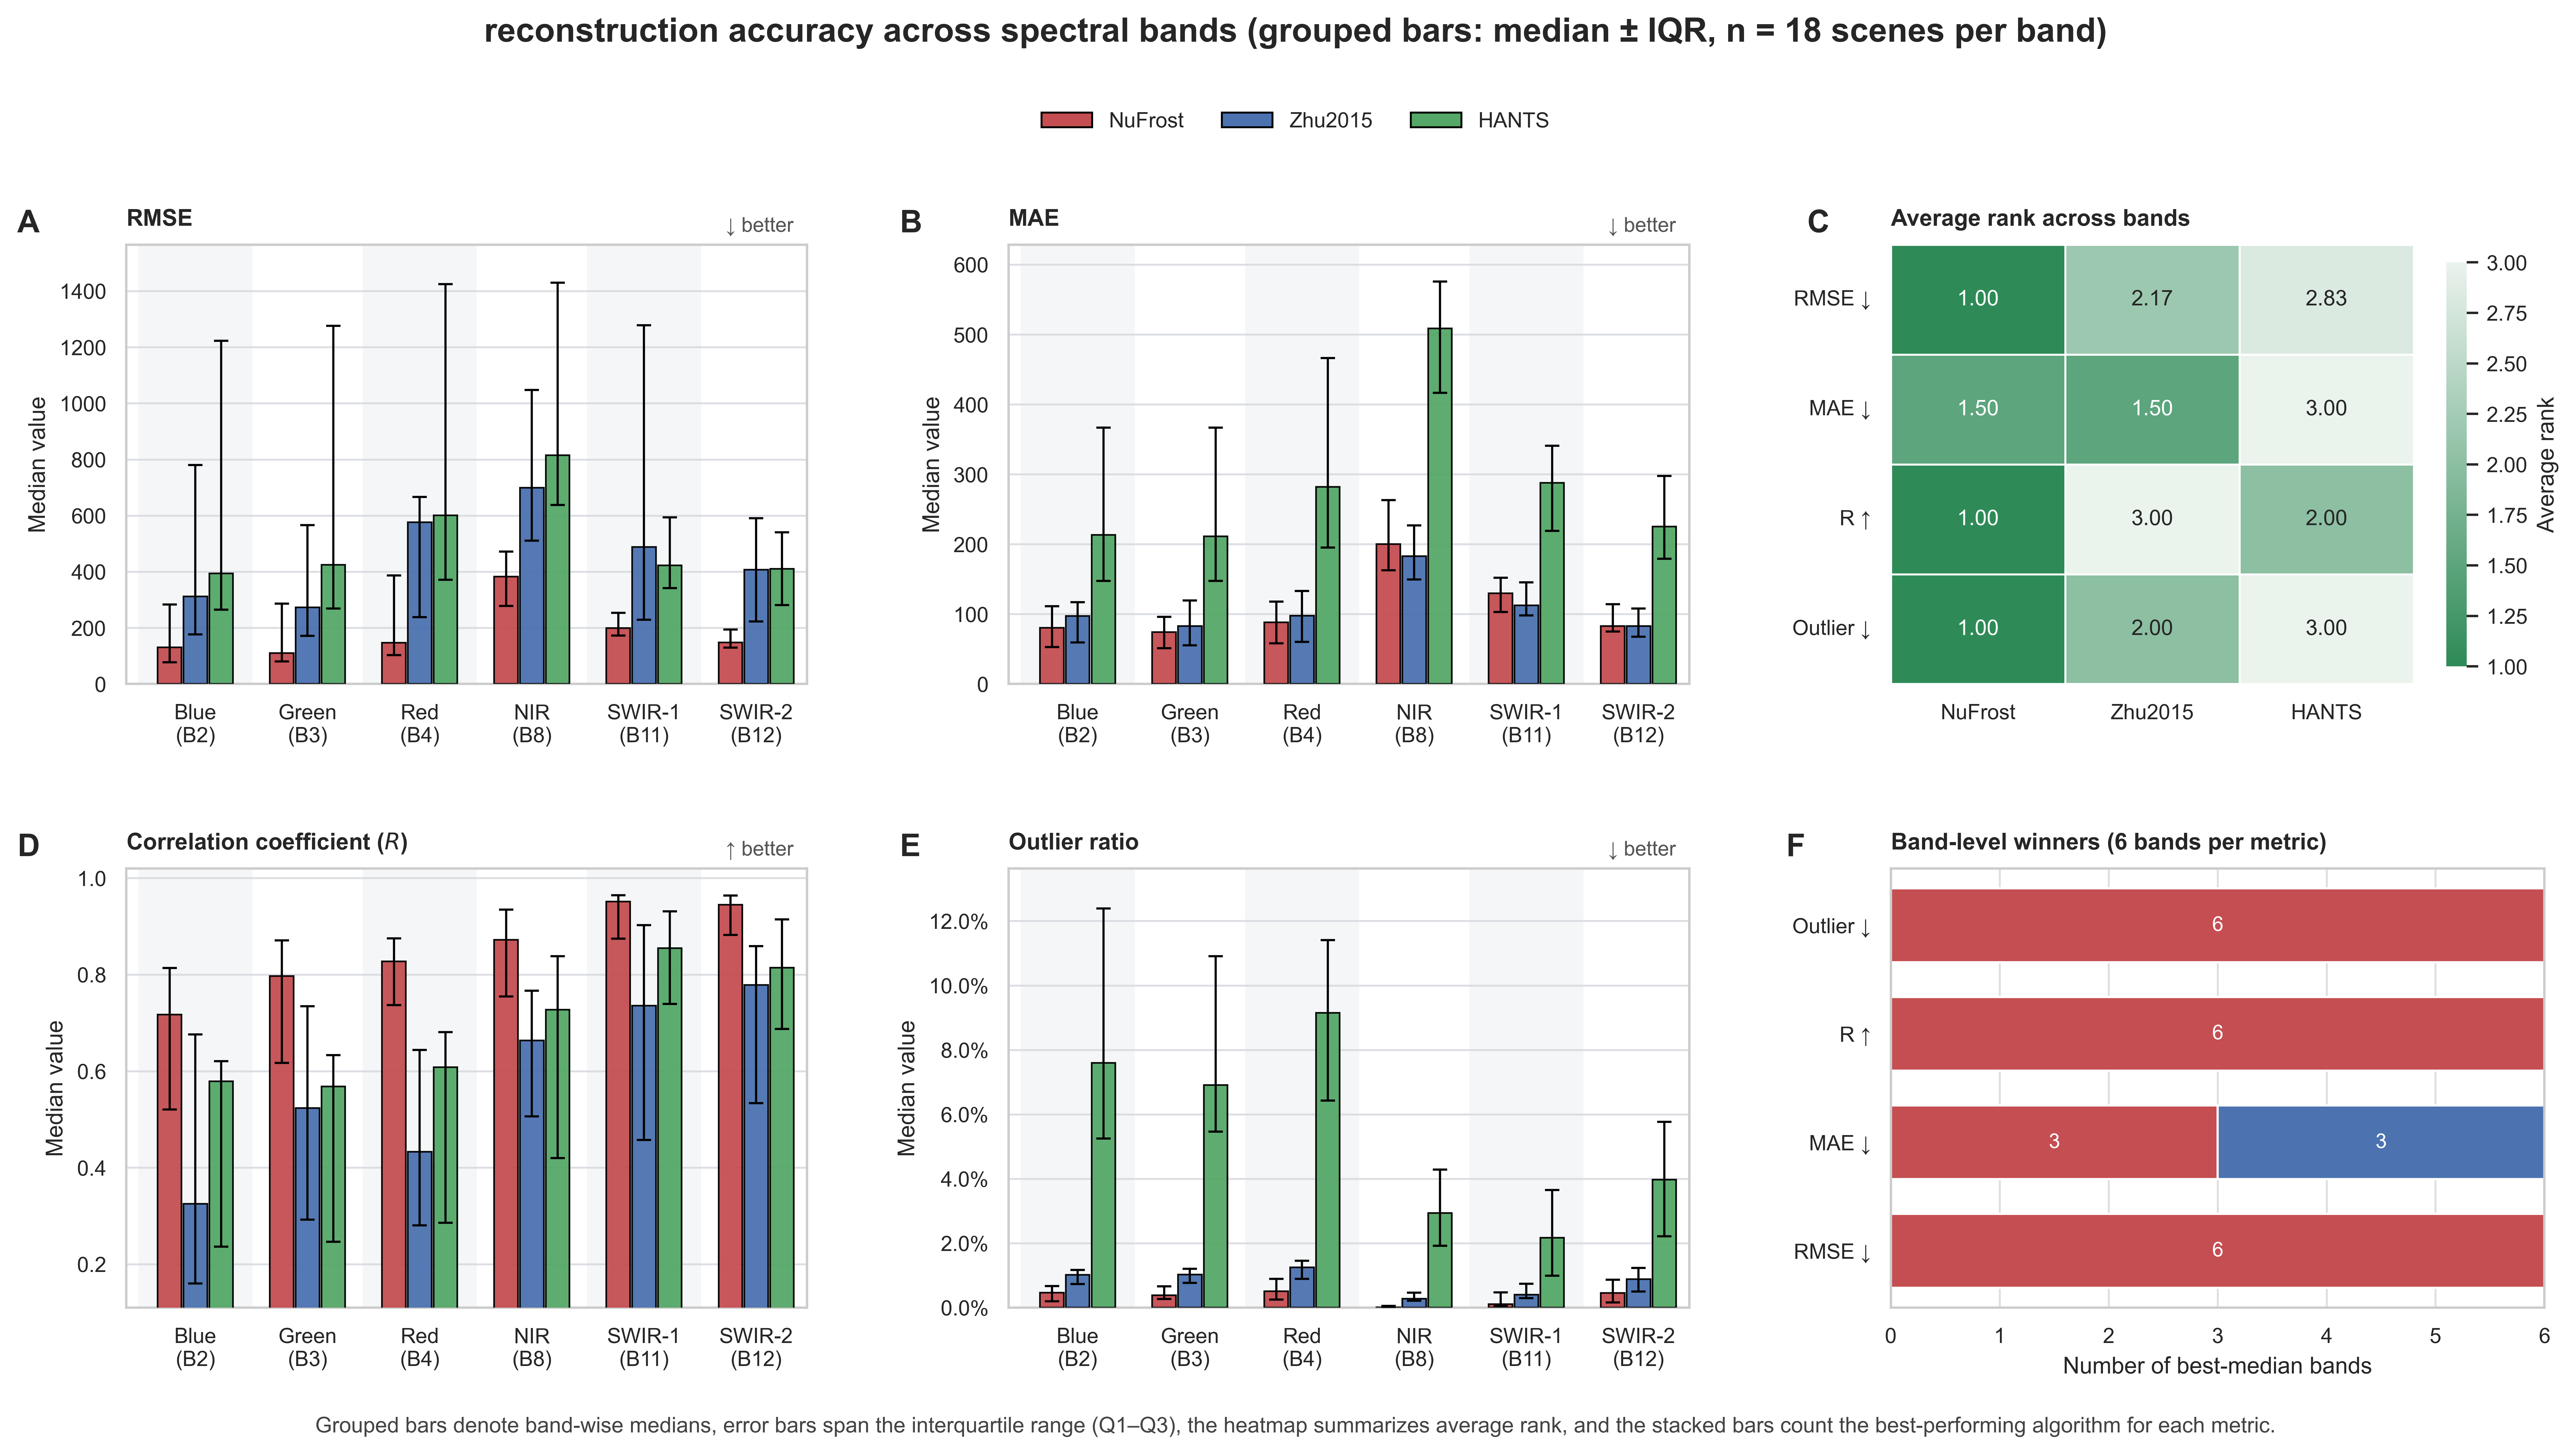
\includegraphics[width=\textwidth]{figures/accuracy.png}
% \hfil
\caption{Comparison of reconstruction accuracy across spectral bands for NUFROST, Zhu2015, and HANTS. Panels report the aggregated performance of the three methods in terms of RMSE, MAE, Pearson correlation coefficient $R$, and outlier ratio. Error bars summarize the variability across evaluated scenes, and the heatmap and stacked summary indicate band-level ranking consistency across the reported metrics.}
\label{fig_sim}
\end{figure*}

\subsection{Experimental Setup}
The experiments were conducted on multiple Sentinel-2 Harmonized AOI time-series cubes covering scenes with substantial cloud contamination and irregular temporal sampling. Each AOI was processed independently, and all compared methods were applied to the same input observations, target pixels, and evaluation masks to ensure a fair comparison. Unless otherwise stated, the same pool of valid observations was used for all methods, and the reported results were aggregated across all evaluated AOIs and spectral bands.

The 15 AOI scenes were intentionally distributed across diverse geographic and ecological settings, including the Tibetan Plateau, southwestern mountainous regions, basin and plain areas, and humid subtropical to tropical environments. This sampling strategy was designed to cover strong variations in topographic complexity, cloud contamination, vegetation phenology, and observation regularity. As a result, the evaluation tests whether NUFROST generalizes not only to difficult mountain scenes with persistent gaps and outliers, but also to relatively stable agricultural and low-relief regions.

To rigorously test the resilience of the algorithms to missing data, we designed two complementary simulation settings:
\begin{itemize}
    \item \textbf{Random point masking (sparse-observation simulation):} For pixels with a sufficient number of valid observations, we randomly removed valid samples from the original spatiotemporal cube and used the remaining irregular observations to predict the masked values. This setting evaluates the ability of each method to recover missing observations when the available time series is sparse but still distributed across the observation period.
    \item \textbf{Continuous gap simulation (prolonged cloud-cover simulation):} To emulate persistent cloud cover and seasonal observation outages, we inserted artificial continuous missing intervals into valid pixel-wise time series and then reconstructed the masked segment from the remaining observations. Gap lengths ranged from short interruptions to long missing periods, allowing us to test the stability of each method under increasingly severe temporal discontinuity. To quantify gap severity, we define a gap index as:
    \begin{equation}
    \label{eq:gap_index}
    I_{gap}=\frac{1}{N^2}\sum_i{l_i^2}
    \end{equation}
    \begin{equation}
    \label{eq:gap_index_periodic}
    I_{periodic} = \frac{1}{N^2}\left|\sum_i l_i e^{j2\pi\tau_i}\right|^2
    \end{equation}
    where $N$ is the total sequence length, $l_i$ is the duration of the $i$-th gap, and $\tau_i$ denotes the temporal position of that gap. In practice, we use these indices to organize the simulated-gap experiments from relatively mild to highly challenging missing-data cases.
\end{itemize}

For all experiments, NUFROST, Zhu2015, and HANTS were evaluated on the same masked targets. Hyperparameters for each method were kept fixed throughout the comparison in order to avoid case-specific tuning. This protocol emphasizes robustness under a unified evaluation pipeline rather than per-scene manual optimization. Final summaries were reported over repeated masking experiments and aggregated across ROIs to reduce sensitivity to any single random split.



\subsection{Evaluation Metrics}
The predicted reflectance values were compared against the original valid observations treated as reference values. We report four complementary metrics to assess both reconstruction accuracy and robustness:
\begin{itemize}
    \item \textbf{Root Mean Square Error (RMSE):} Measures overall reconstruction error and penalizes large deviations more strongly.
    \item \textbf{Mean Absolute Error (MAE):} Measures the average absolute prediction error and is less sensitive to isolated extreme residuals than RMSE.
    \item \textbf{Pearson correlation coefficient ($R$):} Measures the consistency between reconstructed and reference temporal variation.
    \item \textbf{Outlier ratio:} Measures the fraction of predictions whose errors exceed a robust tolerance bound, thereby reflecting the stability of a method in the presence of residual contamination and difficult temporal gaps.
\end{itemize}

Lower RMSE, MAE, and outlier ratio indicate better performance, whereas a higher $R$ indicates better agreement with the reference trajectory. In the result summaries, we report aggregated statistics across ROIs and bands rather than relying on a single representative scene, so that the comparison reflects overall behavior under heterogeneous observation conditions.

\subsection{Reconstruction Accuracy}

The overall reconstruction accuracy of NUFROST, Zhu2015, and HANTS is visualized in Fig.~\ref{fig_sim}. Across all evaluated Sentinel-2 scenes and spectral bands, NUFROST achieved the lowest median RMSE and MAE. Specifically, NUFROST obtained an RMSE of~199.8 and an MAE of~100.7, compared with Zhu2015 (RMSE~492.8, MAE~108.0) and HANTS (RMSE~488.9, MAE~288.2). In terms of temporal consistency, NUFROST attained the highest median Pearson $R$ coefficient (0.852 vs.\ 0.558 for Zhu2015 and 0.635 for HANTS). Furthermore, NUFROST exhibited the smallest outlier ratio (0.32\%), indicating superior robustness against residual contamination, whereas Zhu2015 and HANTS produced ratios of 0.78\% and 5.25\%, respectively.

The per-band analysis reveals that NUFROST consistently outperformed the baseline methods across all six Sentinel-2 bands (B2, B3, B4, B8, B11, B12). The improvement is particularly pronounced in the visible bands (B2, B3, B4) where atmospheric scattering and residual cloud effects are more severe. For instance, in the blue band (B2) NUFROST reduced the median RMSE to 130.1 (vs. 312.3 for Zhu2015 and 394.0 for HANTS) while increasing $R$ to 0.717 (vs. 0.325 and 0.579). The near-infrared and short-wave infrared bands (B8, B11, B12) also benefited from NUFROST's step-preserving frequency regularization, with $R$ values exceeding 0.87 in all three bands. These results confirm that NUFROST's direct spectral estimation from irregular samples, combined with frequency-tiered harmonic fitting and sparse step reconstruction, delivers more accurate and stable reconstructions than conventional interpolation-based or harmonic-fitting approaches.

\subsection{Sparse-Observation Resilience}
To evaluate the resilience of each algorithm under sparse temporal sampling, we conducted random point-masking experiments where valid observations were removed from otherwise complete pixel-wise time series. NUFROST degrades more gracefully than the baseline methods as the number of retained observations decreases. Although all methods become less accurate under severe sparsity, NUFROST preserves a more stable error profile, whereas Zhu2015 and HANTS exhibit a sharper loss of reconstruction quality as temporal support becomes limited.

The advantage of NUFROST stems from its ability to estimate dominant frequencies directly from irregular samples via NUFFT, avoiding the spectral distortion introduced by interpolation-based regularization. When observations become extremely sparse, the baseline methods have less temporal support for constraining the seasonal trajectory and therefore become more sensitive to model mismatch and residual contamination. NUFROST's frequency-tiered Ridge penalty stabilizes the harmonic component by suppressing unreliable high-frequency coefficients, while the sparse step term provides a local mechanism for persistent changes that would otherwise cause ringing in a purely harmonic model.

\subsection{Continuous-Gap Reconstruction}
Persistent cloud cover often leads to extended periods of missing data, posing a particular challenge for time-series reconstruction. We simulated continuous gaps of varying lengths and evaluated each algorithm's ability to recover the missing segment. NUFROST consistently yields lower gap-filling error and a more stable response as the missing interval grows. The contrast becomes especially clear for more challenging gaps, where Zhu2015 and HANTS are more prone to drift away from the underlying seasonal trajectory while NUFROST better preserves the expected temporal structure.

The robustness of NUFROST under prolonged missing intervals is attributed to three key design elements. First, the NUFFT-based spectrum estimation does not rely on evenly spaced samples, so the spectral peaks corresponding to annual and semi-annual cycles can still be reliably identified even when a whole season is missing. Second, the frequency-tiered Ridge terms in Eq.~\ref{eq:objective} improve the conditioning of the harmonic coefficient update, enhancing numerical stability and reducing the wild oscillations that often plague least-squares solutions in rank-deficient scenarios. Third, the group fused-lasso term discourages the model from using globally oscillatory high-frequency components to approximate localized changes. Consequently, NUFROST can reconstruct plausible temporal trajectories through long data gaps without introducing artificial spikes or unrealistic seasonal patterns.

\section{Conclusion}

This paper presented NUFROST, a robust reconstruction framework for irregularly sampled optical remote sensing time series. By combining the Non-Uniform Fast Fourier Transform with frequency-tiered harmonic fitting and sparse step reconstruction, NUFROST addresses three fundamental challenges in temporal reconstruction: spectral distortion introduced by interpolation-based preprocessing, high-frequency ringing caused by over-flexible harmonic fitting, and cross-band inconsistency caused by residual cloud contamination.

The NUFFT enables direct spectrum estimation from irregularly sampled observations without temporal regularization, preserving the true spectral characteristics of the signal. The hybrid frequency selection strategy, combining prior phenological knowledge with data-driven spectral peak detection and parabolic refinement, ensures robust identification of dominant frequencies across diverse observation conditions. The proposed reconstruction objective separates smooth harmonic phenology from sparse persistent steps, while joint multi-band outlier screening and frequency-tiered Ridge regularization improve numerical stability and reduce color speckle under severe temporal gaps.

Experiments on Sentinel-2 Harmonized time series across 15 ROI scenes and six spectral bands demonstrate that NUFROST outperforms both HANTS and Zhu2015 in terms of RMSE, MAE, Pearson correlation, and outlier ratio. The advantage is consistent across spectral bands and particularly pronounced under sparse-observation and continuous-gap scenarios.

Future work may extend NUFROST to multi-sensor fusion scenarios and explore adaptive hyperparameter selection based on per-pixel observation characteristics.

\begin{thebibliography}{16}

\bibitem{ref1}
C. G\'{o}mez, J. C. White, and M. A. Wulder, ``Optical remotely sensed time series data for land cover classification: A review,'' \textit{ISPRS Journal of Photogrammetry and Remote Sensing}, vol. 116, pp. 55--72, 2016.

\bibitem{ref2}
Z. Zhu and C. E. Woodcock, ``Continuous change detection and classification of land cover using all available Landsat data,'' \textit{Remote Sensing of Environment}, vol. 144, pp. 152--171, 2014.

\bibitem{ref3}
J. Verbesselt, R. Hyndman, G. Newnham, et al., ``Detecting trend and seasonal changes in satellite image time series,'' \textit{Remote Sensing of Environment}, vol. 114, no. 1, pp. 106--115, 2010.

\bibitem{ref4}
J. A. Fessler and B. P. Sutton, ``Nonuniform fast Fourier transforms using min-max interpolation,'' \textit{IEEE Transactions on Signal Processing}, vol. 51, no. 2, pp. 560--574, 2003.

\bibitem{ref5}
A. V. Oppenheim, A. S. Willsky, and S. H. Nawab, \textit{Signals \& Systems}, 2nd ed. Upper Saddle River, NJ, USA: Prentice Hall.

\bibitem{ref6}
A. H. Barnett, J. Magland, and L. af Klinteberg, ``A parallel nonuniform fast Fourier transform library based on an `exponential of semicircle' kernel,'' \textit{SIAM Journal on Scientific Computing}, vol. 41, no. 5, pp. C479--C504, 2019.

\bibitem{ref7}
Z. Zhu, J. Zhang, Z. Yang, et al., ``Continuous monitoring of land disturbance based on Landsat time series,'' \textit{Remote Sensing of Environment}, vol. 238, Art. no. 111116, 2020.

\bibitem{ref8}
P. J. Huber, ``Robust estimation of a location parameter,'' \textit{The Annals of Mathematical Statistics}, vol. 35, no. 1, pp. 73--101, 1964.

\bibitem{ref9}
A. E. Hoerl and R. W. Kennard, ``Ridge regression: Biased estimation for nonorthogonal problems,'' \textit{Technometrics}, vol. 12, no. 1, pp. 55--67, 1970.

\bibitem{ref10}
G. J. Roerink, M. Menenti, and W. Verhoef, ``Reconstructing cloudfree NDVI composites using Fourier analysis of time series,'' \textit{International Journal of Remote Sensing}, vol. 21, no. 9, pp. 1911--1917, 2000.

\bibitem{ref11}
R. E. Kennedy, Z. Yang, and W. B. Cohen, ``Detecting trends in forest disturbance and recovery using yearly Landsat time series: 1. LandTrendr temporal segmentation algorithms,'' \textit{Remote Sensing of Environment}, vol. 114, no. 12, pp. 2897--2910, 2010.

\bibitem{ref12}
V. J. Pasquarella, P. Arevalo, K. H. Bratley, et al., ``Demystifying LandTrendr and CCDC temporal segmentation,'' \textit{International Journal of Applied Earth Observation and Geoinformation}, vol. 110, Art. no. 102806, 2022.

\bibitem{ref13}
H. Yin, B. Tan, D. Frantz, et al., ``Integrated topographic corrections improve forest mapping using Landsat imagery,'' \textit{International Journal of Applied Earth Observation and Geoinformation}, vol. 108, Art. no. 102716, 2022.

\bibitem{ref14}
Z. Zhu, C. E. Woodcock, C. Holden, et al., ``Generating synthetic Landsat images based on all available Landsat data: Predicting Landsat surface reflectance at any given time,'' \textit{Remote Sensing of Environment}, vol. 162, pp. 67--83, 2015.

\bibitem{ref15}
R. Tibshirani, M. Saunders, S. Rosset, J. Zhu, and K. Knight, ``Sparsity and smoothness via the fused lasso,'' \textit{Journal of the Royal Statistical Society: Series B}, vol. 67, no. 1, pp. 91--108, 2005.

\bibitem{ref16}
S. Boyd, N. Parikh, E. Chu, B. Peleato, and J. Eckstein, ``Distributed optimization and statistical learning via the alternating direction method of multipliers,'' \textit{Foundations and Trends in Machine Learning}, vol. 3, no. 1, pp. 1--122, 2011.

\end{thebibliography}

\end{document}
